\documentclass[12pt,a4paper]{report}
\usepackage[a4paper,left=1in,right=1in,top=1in,bottom=1in]{geometry}

\usepackage{listings}
\usepackage{color}
 
\definecolor{codegreen}{rgb}{0,0.6,0}
\definecolor{codegray}{rgb}{0.5,0.5,0.5}
\definecolor{codepurple}{rgb}{0.58,0,0.82}
 
\lstdefinestyle{mystyle}{ 
    commentstyle=\color{codegreen},
    keywordstyle=\color{magenta},
    numberstyle=\tiny\color{codegray},
    stringstyle=\color{codepurple},
    basicstyle=\normalfont\ttfamily,
    breakatwhitespace=false,         
    breaklines=true,                 
    captionpos=b,                    
    keepspaces=true,                 
    numbers=left,                    
    numbersep=5pt,                  
    showspaces=false,                
    showstringspaces=false,
    showtabs=false,                  
    tabsize=3
}
 
\lstset{style=mystyle}

\usepackage{amssymb}
\usepackage{booktabs}
\usepackage{setspace}
\usepackage{tabularx}
\usepackage[pdftex]{graphicx} %for embedding images
\usepackage{url} %for proper url entries
\usepackage[bookmarks, colorlinks=false, pdfborder={0 0 0}, pdftitle={Quad-Pi Report}, pdfauthor={Tushaar G.}, pdfsubject={Minor Project Report}, pdfkeywords={RPi, Parallel, Emotion, OpenCV}]{hyperref} %for creating links in the pdf version and other additional pdf attributes, no effect on the printed document
\usepackage[final]{pdfpages} %for embedding another pdf, remove if not required

%Page Border
\usepackage{pgf}
\usepackage{pgfpages}

\pgfpagesdeclarelayout{boxed}
{
  \edef\pgfpageoptionborder{0pt}
}
{
  \pgfpagesphysicalpageoptions
  {%
    logical pages=1,%
  }
  \pgfpageslogicalpageoptions{1}
  {
    border code=\pgfsetlinewidth{1pt}\pgfstroke,%
    border shrink=\pgfpageoptionborder,%
    resized width=.88\pgfphysicalwidth,%
    resized height=.88\pgfphysicalheight,%
    center=\pgfpoint{.5\pgfphysicalwidth}{.5\pgfphysicalheight}%
  }%
}
\pgfpagesuselayout{boxed}
\setlength{\parindent}{1cm}

\begin{document}
\linespread{1.5}
\renewcommand\bibname{References} %Renames "Bibliography" to "References" on ref page

%include other pages
\pagenumbering{gobble}
\begin{titlepage}

\begin{center}
\textup{\small \textit{Project Report On}}\\

% Title
\Large \textbf {Real-Time Emotion Detection using Quad-Pi}\\[0.4in]

% Submitted by
\normalsize \textit{Submitted by} \\
\begin{table}[h]
\centering
\bgroup
\def\arraystretch{1.4}
\begin{tabular}{lr}
\textbf{15IT117} & \textbf{Tushaar Gangarapu} \\
\textbf{15IT114} & \textbf{Bharath A. Kinnal} \\ 
\textbf{15IT213} & \textbf{Jyoti Prakash Sahoo} \\
\end{tabular}
\egroup
\end{table}

\textbf{VI Semester B.Tech (IT)}\\[0.3in]

\textit{Under the guidance of}\\\vspace{3mm}
{\textbf{Dr. Geetha V}}\\
{\textbf{Department of IT, NITK Surathkal}}\\[0.3in]

       \small \emph{in partial fulfillment for the award of the degree\\\vspace{2mm} of}
        \vspace{.2in}

       {\bf Bachelor of Technology} \\\vspace{2mm} \textit{in} \\\vspace{2mm} {\bf Information Technology} \\\vspace{2mm} \textit{at}\\[0.2in]

% Bottom of the page

\includegraphics[width=0.18\textwidth]{images/logo}\\
\Large{Department of Information Technology}\\
\normalsize
\textsc{National Institute of Technology Karnataka, Surathkal}\\
March 2018 \\
\vspace{0.2cm}

\end{center}

\end{titlepage}

\newpage
\thispagestyle{empty}

\begin{center}

\huge{Department of Information Technology}\\[0.5cm]
\normalsize
\textsc{National Institute of Technology Karnataka, Surathkal}\\[2.0cm]

\emph{\LARGE Mid Semester Evaluation (March 2018)}\\[2cm]
\end{center}
\begin{table}[h]
\centering
\bgroup
\def\arraystretch{1.5}
\begin{tabular}{ll}
\textbf{Course Code:} & IT399 \\
\textbf{Course Title:} & Minor Project \\ 
\textbf{Title of the Project:} & Real-Time Emotion Detection using Quad-Pi \\
\textbf{Project Group:} &
\end{tabular}
\egroup
\end{table}

\begin{table}[h]
\centering
\bgroup
\def\arraystretch{1.5}
\begin{tabular}{lcr}
Register No. & Name of Student & Signature (with date) \\ \\ \hline
\\
15IT117 & Tushaar Gangarapu & \line(1,0){100} \\ 
15IT114 & Bharath A. Kinnal &  \line(1,0){100} \\
15IT213 & Jyoti Prakash Sahoo & \line(1,0){100}  \\
\end{tabular}
\egroup
\end{table}

\vfill


% Bottom of the page
\noindent
\bgroup
\def\arraystretch{1.5}
\begin{tabular}[t]{@{}l} 
Project Guide: Dr. Geetha V \\
Signature (with date): \line(1,0){100}
\end{tabular}
\hfill% move it to the right
\begin{tabular}[t]{r@{}}
Place: NITK, Surathkal \\
Date: \today
\end{tabular}
\egroup
\newpage
\thispagestyle{empty}

\begin{center}

\huge{Department of Information Technology}\\[0.5cm]
\normalsize
\textsc{National Institute of Technology Karnataka, Surathkal}\\[2.0cm]

\emph{\LARGE Declaration}\\[2cm]
\end{center}
\normalsize We hereby declare that the Project Work Report entitled ``\textbf{Real-Time Emotion Detection using Quad-Pi}'' which is being submitted to {\bf National Institute of Technology Karnataka, Surathkal} in accordance with the completion of the minor project for the degree of {\bf Bachelor of Technology} in {\bf Information Technology} is a bonafide report of the work carried out by us. \\[1.0cm]

\begin{table}[h]
\centering
\bgroup
\def\arraystretch{1.2}
\begin{tabular}{lr}
Register No. & Name of Student \\ \\ \hline
\\
15IT117 & Tushaar Gangarapu \\ 
15IT114 & Bharath A. Kinnal \\
15IT213 & Jyoti Prakash Sahoo \\
\end{tabular}
\egroup
\end{table}

\vfill


% Bottom of the page
\begin{flushleft}
Department of Information Technology \\
Place: NITK, Surathkal \\
Date: \today
\end{flushleft}

\newpage
\thispagestyle{empty}

\begin{center}

\huge{Department of Information Technology}\\[0.5cm]
\normalsize
\textsc{National Institute of Technology Karnataka, Surathkal}\\[2.0cm]

\emph{\LARGE Certificate}\\[2cm]
\end{center}
\normalsize This is to certify that this is a bonafide record of the project entitled ``\textbf{Real-Time Emotion Detection using Quad-Pi}'' presented by the students whose names are given below during VI semester 2018 in partial fulfilment of the requirements of the degree of Bachelor of Technology in Computer Science and Engineering.\\[1.0cm]

\begin{table}[h]
\centering
\bgroup
\def\arraystretch{1.2}
\begin{tabular}{lr}
Register No. & Name of Student \\ \\ \hline
\\
15IT117 & Tushaar Gangarapu \\ 
15IT114 & Bharath A. Kinnal \\
15IT213 & Jyoti Prakash Sahoo \\
\end{tabular}
\egroup
\end{table}

\vfill


% Bottom of the page
\noindent
\begin{tabular}[t]{@{}l} 
\\
Date: \today
\end{tabular}
\hfill% move it to the right
\begin{tabular}[t]{r@{}}
Dr. Geetha V \\
(Project Guide)
\end{tabular}

\cleardoublepage
%\pagebreak
\phantomsection
\addcontentsline{toc}{chapter}{Acknowledgements}
\chapter*{Acknowledgments}
We take this opportunity to express our deepest gratitude and appreciation to all those who have helped us directly or indirectly towards the successful completion of this project. \par
First and foremost, we would like to express our sincere appreciation and gratitude to our esteemed guide \textit{Dr. Geetha V}, Department of Information Technology, NITK Surathkal for her insightful advice, encouragement, guidance, critics, and valuable suggestions throughout the course of our project work. Without her continued support and interest, this thesis would not have been the same as presented here.\par
We would like to take this opportunity to express our thanks towards all the teaching and non-teaching staff in the Department of Information Technology for their invaluable support in this semester of our study. We are also grateful to all our classmates for their  invaluable suggestions. \par
Finally, we thank God Almighty for his blessings without which the completion of this project work would not have been possible.

\vfill

% Bottom of the page
\noindent
\begin{tabular}[t]{@{}l} 
\\
\today \\
{National Institute of Technology Karnataka}\
\end{tabular}
\hfill% move it to the right
\begin{tabular}[t]{r@{}}
Tushaar Gangarapu \\
Bharath A. Kinnal \\
Jyoti Prakash Sahoo
\end{tabular}
\vspace{2in}
\begin{abstract}

In present day technology human-machine interaction is growing in demand and machine needs to understand human gestures and emotions. If a machine can identify human emotions, it can understand human behavior better, thus improving the \textit{task efficiency}. Emotions can understand by text, vocal, verbal and facial expressions (speech can also be used). Facial expressions play big role in judging emotions of a person. It is found that limited work is done in field of real time emotion recognition using facial images. In the base paper \cite{suja2016}, they proposed a method for real time emotion recognition from facial image. The proposed method used three steps face detection using Haar cascade, features extraction using Active shape Model(ASM) and Adaboost classifier for classification of five emotions anger, disgust, happiness, neutral and surprise. Implementation of emotion recognition at real time on Raspberry Pi II is achieved at real time. This process is \textit{parallelized} using Quad-Pi (four Raspberry Pi).

\end{abstract} 


\pagenumbering{roman} %numbering before main content starts
\tableofcontents
\listoffigures
\listoftables

\newpage
\pagenumbering{arabic} %reset numbering to normal for the main content

\chapter{Introduction}

In present day technology human-machine interaction is growing in demand and machine needs to understand human gestures and emotions. If machine can identify human emotion, it can understand human behavior better, thus improving the task efficiency. It can serve as a vital measurement tool for behavioral science, socially intelligent software can be developed which can be used for robots. Emotions are the strong feelings which are governed by the surroundings and play a great role in daily task like decision making, learning, attention, motivation, coping, perception, planning, cognition, reasoning and many more, which leads to emotion recognition a big research field. Emotion recognition can be done by text, vocal, verbal and facial expression. Facial expression analysis is one of the most important components for emotion recognition. Facial emotion recognition from 2D images is well studied field but lack of real-time method that estimates features even low quality images. Most of the work are based on frontal view images of the faces.\par
The method proposed is a real-time emotion recognition system that recognizes basic emotions like anger, disgust, happiness, surprise and neutral using CMU MultiPIE database consisting 2D images with different illumination and poses. The software system developed using our proposed method is deployed on Raspberry Pi II as it can be used with robots as the size of Raspberry Pi II is very small, lightweight and very less power supply is needed for it. As a result it can be mounted over any robot very easily and can be used for many applications such as surveillance security, monitoring senior citizen or children at home, monitoring critical patients in ICU, for customer satisfaction and many more.

\section{Motivation}

If machines can identify human emotions, it can understand human behaviour better which   improves task efficiency. Emotions greatly affect decision making, learning, attention, motivation, coping, planning, cognition, reasoning etc. Facial emotion detection from 2D images is well studied field but lack of real-time method to estimate features gives the necessity to develop a method for the same Parallelization of the real-time process, which might lead to higher speeds keeping accuracy at it peak.
\chapter{Literature Review}

\section{Background and Recent Work}

\subsection{Real-Time Emotion Detection using RPi2}
- By Suja, P. et al. \cite{suja2016} \\
The methodology in this paper involved the use of Raspberry Pi II and CMU MultiPIE database to detect emotions in real-time. The advantages of this methology was that the execution was done at real-time, and had a high speed and high accuracy. However, it only used the features extracted from facial expressions in the image (Speech was considered under `future work').

\subsection{Image Processing on RPi in Matlab}
- Horak, K. et al. \cite{horak2015} \\
The methodology in this paper involved the use of Raspberry Pi II and Simulink in Matlab to process images with many filters such as the Sobel filter. The advantages of this methology was that the execution was done at real-time, and had a high speed. It also extracted features based on edge, corner, line detection. However, it lead to increase in FPS due to transfer from RPi2 to Simulink.

\subsection{Real-Time Face Recognition using RPi2}
- Viji, A. et al. \cite{viji2017} \\
The methodology in this paper involved the use of Raspberry Pi II, Haar cascade classifier, PCA feature extraction, and Adaboost classification to detect faces in real-time. The advantages of this methology was that the execution was done at real-time, and had a high speed and high accuracy. However, it considers only PCA feature extraction.

\pagebreak

\subsection{Robust Real-Time Face Detection}
- Viola, P. et al. \cite{viola2004} \\
The methodology in this paper involved the use of Haar feature selection to create an internal image, and Adaboost training and Cascading classifiers to detect faces in real-time. The advantages of this methology was that the execution required minimal computation time and had a high detection accuracy. However, real-time conditions (illuminations, non-uniform conditions) were ignored.

\section{Outcomes of Literature Review}
Current state-of-art implementations consider facial expressions to be the primary source of emotion detection. Various methods for feature extraction have been used in the past like ASM, PCA which employ geometric-based feature detection. Processing on Raspberry Pi can give speeds upto 100ms and Viola-Jones feature detection gives about 95\% accuracy. Current state-of-art implementations do not consider parallelization of the process. 

\section{Problem Statement}
Face detection, feature extraction, ad finally classification of an image to a particular recognizable emotion. Also implementing the same using a parallel (master-slave) model using Quad-Pi (four RPi3).

\section{Research Objectives}
\begin{itemize}
\item To develop emotion recognition from facial images to simulate and experiment in near real-time environment, programming the Raspberry Pi III, deals with Image Processing (cropping and face extraction), feature extraction from grayscale face image extraction, and classify using Adaptive Boosting classifier trained with CMU MultiPIE database
\item Use Quad-Pi (four RPi3) to implement master-slave parallel processing model to the deployed application.
\end{itemize}

\chapter{Methodology}

\section{System Architecture}
The following components form the system architecture:
\begin{itemize}
\item Raspberry Pi III (Model B)
\item Raspbian Stretch OS
\item Ubuntu 16.04 OS
\item Ethernet Crossover Cable
\item SD Card
\item Adapter for Raspberry Pi III
\end{itemize}
\section{Methodology}

\subsection{Input}
For real-time simulations, input is taken from webcam (further development would be to use a mobile robot) to dynamically recognize emotions, serves as input to Raspberry Pi III.

\subsection{RPi3 Processing}
Pre-Processing for Facial Feature Extraction is the beginning processing unit for RPi3 processing. Viola-Jones \cite{viola2004} face detection technique is used to detect the facial image. Viola-Jones used Haar wavelet concept to develop integral image to detect face. Haar features consider the different intensity of values of adjacent rectangular region as different area of face has different value of intensity from other region. After detection, facial image is saved for further processing and non-face area is removed. 

\subsection{Image Processing}
Image is cropped according to required size and converted in gray image. This cropped image is used as input to \textit{Sobel filter} for smoothing to remove the noise.

\subsection{Feature Extraction}
Feature extraction is based on geometric approach for which Active Shape Model (ASM) is used. ASM automatic fiducial point location algorithm is applied first to a facial expression image, and then Euclidean distances between center gravity coordinate and the annotated fiducial points coordinates of the face image are calculated. Extract geometric deformation difference features between a person's neutral expression and the other basic expressions. Compare with shape model to extract feature points of input facial image.

\subsection{Classification}
This is done by adaptive boosting classifier (AdaBoost). AdaBoost is a powerful learning concept that provides a solution to supervised classification learning task. It combines the performance of many weak classifiers to produce a powerful committee. AdaBoost is a flexible classifier which can be combined with any learning algorithm. It is very simple and easy to perform in which only one parameter i.e., number of iteration is varied to get good accuracy.

\subsection{Quad-Pi Parallelization}
Using master slave the Quad-Pi parallelization perform its operation, Master starts the slave computation, and the slave computation returns the result to the master. No significant dependencies among the slave computations is there. In sense of this research work, \textit{Sobel filter} can be parallelized. In case of multiple people in an image, multiple emotions detection is needed where speeds and task division matter \cite{redmon2016}.

\begin{figure}[htb]
\centering
\includegraphics[scale=0.7]{images/Real-time\ Emotion\ Recognition\ System}
\caption{Real-time Emotion Recognition System}
\label{fig:erSystem}
\end{figure}

\begin{figure}[htb]
\centering
\includegraphics[scale=1]{images/Block\ diagram}
\caption{Block Diagram showing Process Flow of the System}
\label{fig:bd}
\end{figure}

\chapter{Work Done}

\section{Experimental Framework}

\begin{figure}[htb]
\centering
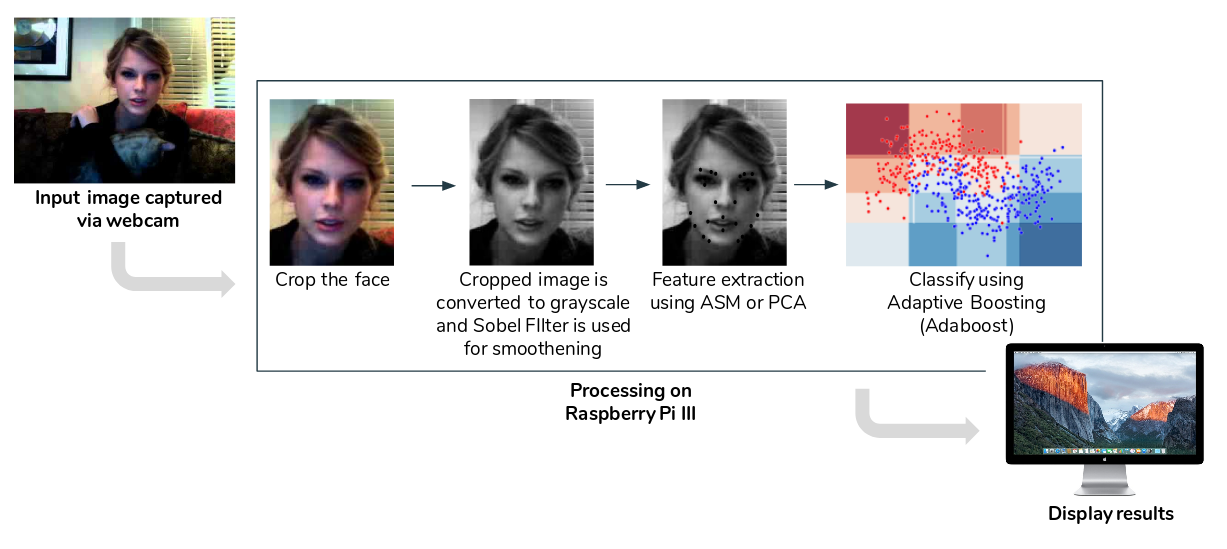
\includegraphics[scale=0.35]{images/model}
\caption{Flow of control from Input to Output to detect `Emotions' (real-time)}
\label{fig:model}
\end{figure}

\section{Work Done (Mid-March 2018)}

\subsection{Capturing Input via Webcam (Linux)}
\begin{lstlisting}[language=python]
pygame.camera.init()
cam = pygame.camera.Camera("/dev/video0", (640, 640))
cam.start()
image = cam.get_image()
pygame.image.save(image, localpath)

try:
    conn = sftp.Connection(host='10.42.0.178', username='pi', password='raspberry')
    conn.put(localpath, remotepath)
    conn.close()
except Exception, e:
    print str(e)
\end{lstlisting}

\subsection{Preprocessing the Image (RPi): Facial Region Extraction}
\begin{lstlisting}[language=python]
def convertToRGB(image):
    return cv2.cvtColor(image, cv2.COLOR_BGR2RGB)

image = cv2.imread(filename)
grayImage = cv2.cvtColor(image, cv2.COLOR_BGR2GRAY)
plt.imshow(grayImage, cmap = "gray")

haarFaceCascade = cv2.CascadeClassifier('training/haarcascade_frontalface_alt.xml')

faces = haarFaceCascade.detectMultiScale(grayImage, scaleFactor = 1.1, minNeighbors = 5)
print "Number of faces found: %s" %(len(faces))

for (x, y, w, h) in faces:
    cv2.rectangle(image, (x, y), (x + w, y + h), (0, 255, 0), 2)
plt.imshow(convertToRGB(image))

def violaJones(filename, trainingFile, scaleFactor = 1.2):
    image = cv2.imread(image_directory + filename)
    grayImage = cv2.cvtColor(image, cv2.COLOR_BGR2GRAY)
    
    haarFaceCascade = cv2.CascadeClassifier(training_directory + trainingFile)
    faces = haarFaceCascade.detectMultiScale(grayImage, scaleFactor = scaleFactor, minNeighbors = 5)
    print "Number of faces found: %s" %(len(faces))

    deleteAllFiles(faces_directory)
    for (x, y, w, h) in faces:
        cv2.rectangle(image,(x, y),(x+w, y+h),(0, 255, 0),2)
        sub_face = image[y : y + h, x : x + w]
        
        faceFile=faces_directory + "face_" + str(y) + ".jpg"
        cv2.imwrite(faceFile, sub_face)
    image = convertToRGB(image)
    return image
\end{lstlisting}


\subsection{Preprocessing the Image (RPi): Sobel Filter}
\begin{lstlisting}[language=python]
image = cv2.imread(filename, cv2.IMREAD_GRAYSCALE)
laplacian = cv2.Laplacian(image, cv2.CV_64F)
sobelX = cv2.Sobel(image, cv2.CV_64F, 1, 0, ksize=5)
sobelY = cv2.Sobel(image, cv2.CV_64F, 0, 1, ksize=5)

def sobelYFilter(directory):
    deleteAllFiles(sobel_directory)
    filelist = [f for f in os.listdir(directory)]
    for f in filelist:
        filename = faces_directory + f

        image = cv2.imread(filename, cv2.IMREAD_GRAYSCALE)
        sobelY = cv2.Sobel(image, cv2.CV_64F, 0, 1, ksize=5)
        
        sobelFile = sobel_directory + f
        cv2.imwrite(sobelFile, sobelY)
        plt.imshow(sobelY)
\end{lstlisting}

\section{Results and Discussion}

\subsection{Capturing on Linux}
\begin{figure}[htb]
\centering

\includegraphics[scale=0.7]{images/capture}
\caption{Capturing through webcam in real-time (different illuminations and non-uniform conditions) with low resolution}
\label{fig:capture}
\end{figure}

\subsection{Viola-Jones on RPi3}
The facial image is detected by using Viola-Jones face detection technique. The integral image is developed by using Haar wavelet concept to detect the face. It consider the different intensity of values of adjacent rectangular regions. The different areas of face have different intensity. Face is detected and pointed by using rectangular box (then cropped). Refer figures \ref{fig:vj1}, \ref{fig:vj2}, \ref{fig:vj3} and \ref{fig:vj4}.

\begin{figure}[htb]
\centering
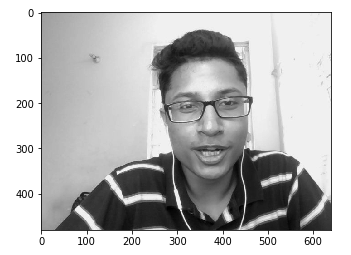
\includegraphics[scale=0.5]{images/vj_img1}
\caption{Converting the input image (from Linux) into grayscale}
\label{fig:vj1}
\end{figure}

\begin{figure}[htb]
\centering
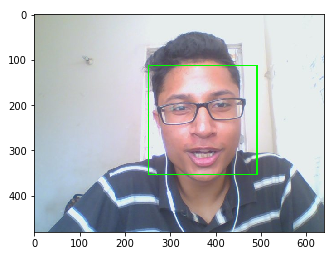
\includegraphics[scale=0.5]{images/vj_img2}
\caption{Face Detection using Haar-Cascade Classifier (of figure \ref{fig:vj1})}
\label{fig:vj2}
\end{figure}

\begin{figure}[htb]
\centering
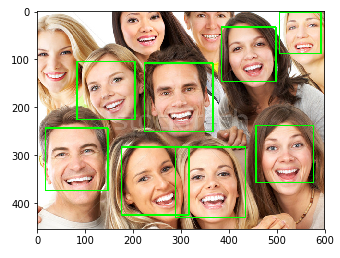
\includegraphics[scale=0.5]{images/vj_img3}
\caption{Capturing multiple faces using Viola-Jones Algorithm (Haar-Cascade)}
\label{fig:vj3}
\end{figure}

\begin{figure}[htb]
\centering

\includegraphics[scale=0.5]{images/vj_img4}
\caption{Crop the facial part and discard the rest of the image (of figure \ref{fig:vj3})}
\label{fig:vj4}
\end{figure}

\subsection{Image Processing on RPi3}
In image preprocessing, image is cropped according to required size and converted in gray image. This cropped image is used as input to Sobel filter for smoothing to remove the noise. Refer figures \ref{fig:ip1}, \ref{fig:ip2}.

\begin{figure}[htb]
\centering
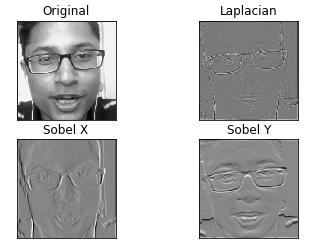
\includegraphics[scale=0.5]{images/ip_img1}
\caption{Crop the facial part and discard the rest of the image (of figure \ref{fig:vj2})}
\label{fig:ip1}
\end{figure}

\begin{figure}[htb]
\centering

\includegraphics[scale=0.5]{images/ip_img2}
\caption{Crop the facial part and discard the rest of the image (of figure \ref{fig:vj4})}
\label{fig:ip2}
\end{figure}
\pagebreak

\section{Individual Contributions}

\begin{itemize}
\item Tushaar Gangarapu (15IT117) -- RPi3 Configuration, Capturing real-time input and directing it to RPi3 for pre-processing and emotion detection.
\item Bharath A. Kinnal (15IT114) -- Use the image obtained and run Haar-Cascade classifier to obtain `facial' region of the image.
\item Jyoti Prakash Sahoo (15IT213) -- Use the facial image and run `Sobel Filter' along \textit{Y-axis} and remove noise.
\end{itemize}
\chapter{Conclusion and Future Work}

Input image is captured through webcam (real-time). Viola-Jones \cite{viola2004} face detection technique is used to detect the facial image. Viola-Jones used Haar wavelet concept to develop integral image to detect face. Haar features consider the different intensity of values of adjacent rectangular region as different area of face has different value of intensity from other region (\textit{haarcascade\_frontalface\_default.xml} for training). After detection, facial image is saved for further processing and non-face area is removed. In image preprocessing, image is cropped according to required size and converted in gray image. This cropped image is used as input to Sobel filter for smoothing to remove the
noise.

\section{Proposed Work Plan of the project}

\begin{table}[h]
\centering
\bgroup
\def\arraystretch{1.5}
\caption{Work Plan through the Course Time and Objectives}
\begin{tabularx}{\linewidth}{X c c c c}
\hline
Milestones & February 2018 & Mid-March 2018 & End-March 2018 & April 2018 \\
\hline
Research and Feasibility study & \checkmark & \checkmark & \checkmark & \checkmark \\
RPi3 configuration with real-time input capturing and pre-processing & & \checkmark & \checkmark & \checkmark \\
Real-time emotion detection (RPi3) & & & \checkmark & \checkmark \\
Master-Slave model (Quad-Pi) & & & & \checkmark \\
\hline
\end{tabularx}
\egroup
\end{table}
\cleardoublepage
%\pagebreak
\phantomsection
\addcontentsline{toc}{chapter}{References}
\begin{thebibliography}{99}

\bibitem{suja2016}Suja, P., \& Tripathi, S. (2016, February). Real-time emotion recognition from facial images using Raspberry Pi II. In Signal Processing and Integrated Networks (SPIN), 2016 3rd International Conference on (pp. 666-670). IEEE.

\bibitem{horak2015}Horak, K., \& Zalud, L. (2015). Image Processing on Raspberry Pi in Matlab. Advances in intelligent systems and computing, 4.

\bibitem{viji2017}Viji, A., \& Pavithra, A. (2017). Real Time Face Recognition using Raspberry Pi II. IJIRSET, Vol. 6, Special Issue 3.

\bibitem{viola2004}Viola, P., \& Jones, M. J. (2004). Robust real-time face detection. International journal of computer vision, 57(2), 137-154.

\bibitem{suk2014}Suk, M., \& Prabhakaran, B. (2014). Real-time mobile facial expression recognition system-a case study. In Proceedings of the IEEE Conference on Computer Vision and Pattern Recognition Workshops (pp. 132-137).

\bibitem{redmon2016}Redmon, J., Divvala, S., Girshick, R., \& Farhadi, A. (2016). You only look once: Unified, real-time object detection. In Proceedings of the IEEE conference on computer vision and pattern recognition (pp. 779-788).

\end{thebibliography}


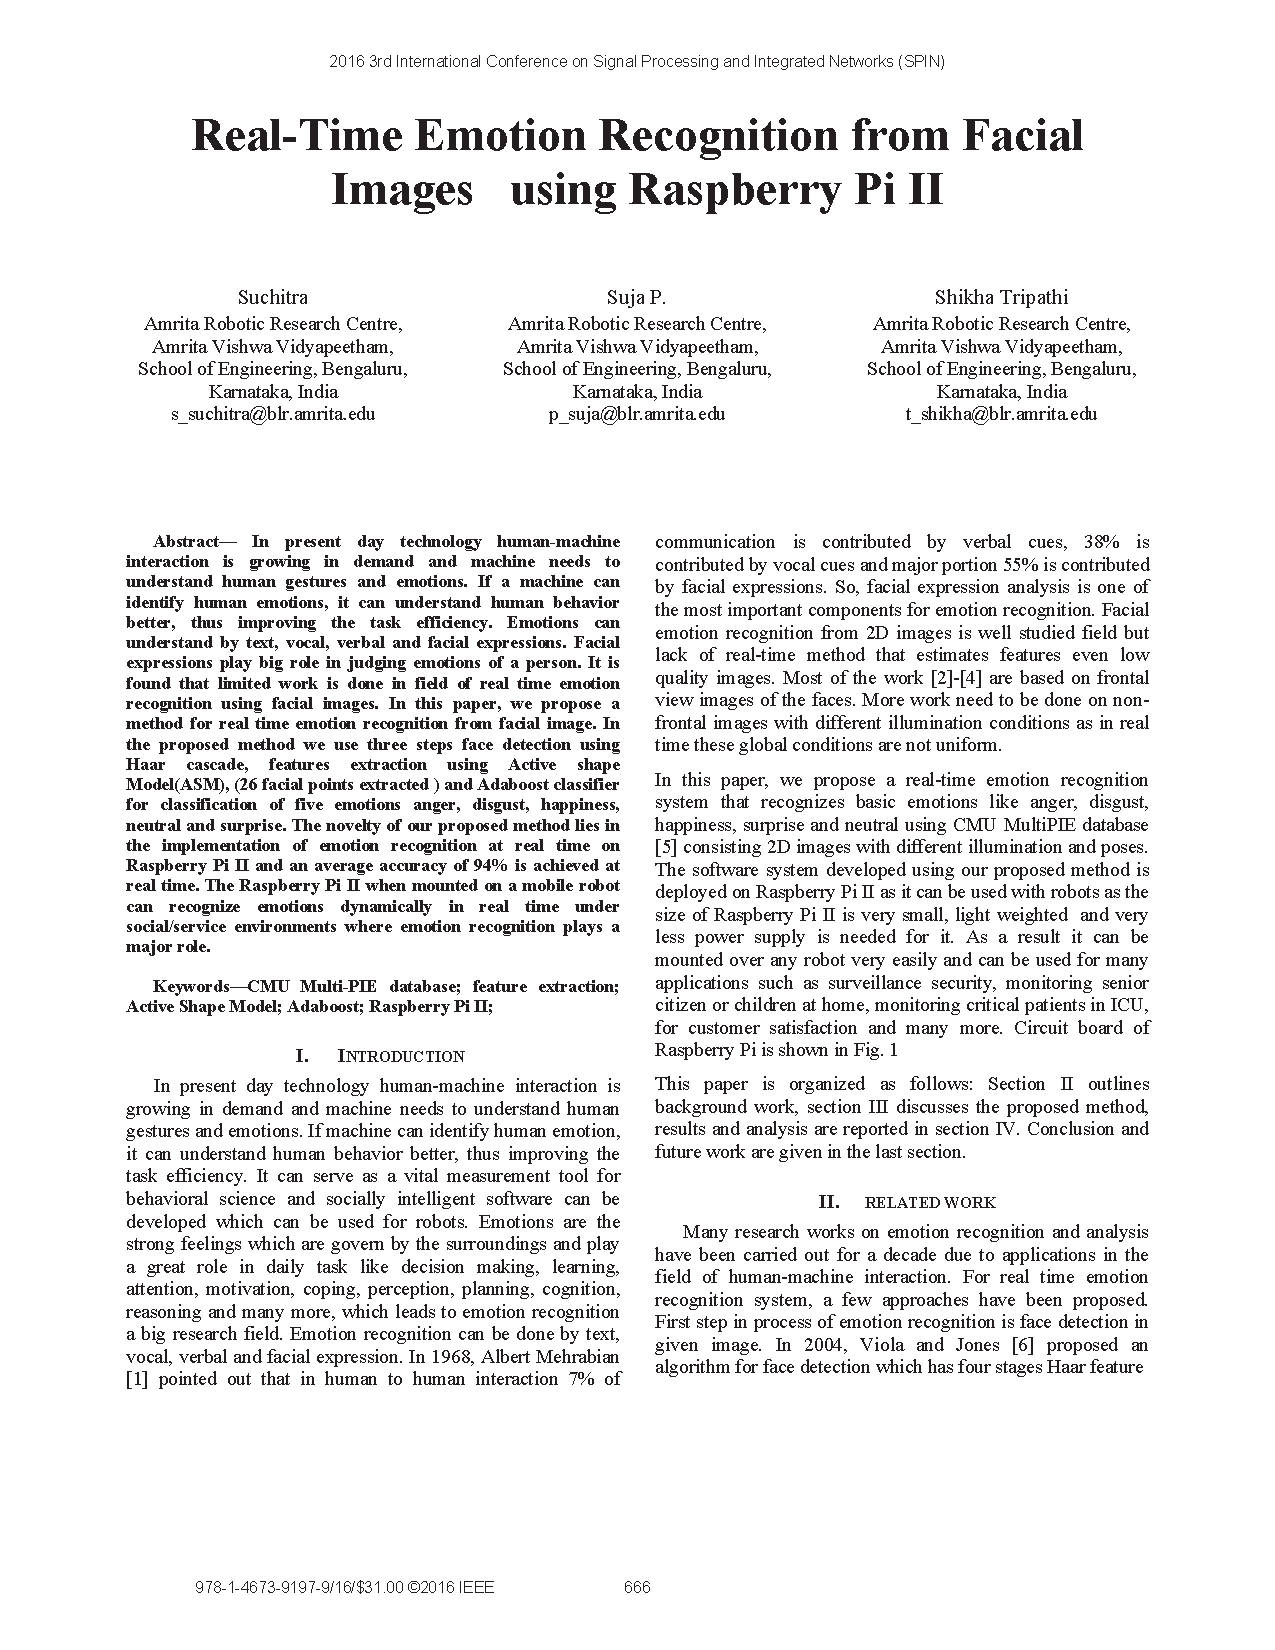
\includepdf[pages=-]{/home/tushaar/Desktop/minor_project/GitHub/references/emotion_recognition_RPi.pdf}
\end{document}
